\section{Les cas d'utilisation}
\label{sec:use-cases}

\paragraph{}
Le seul besoin métier est la validation de fichiers Excel contenant des données utiles à l'accomplissement du travail de l'utilisateur. Toutefois, la mise en place d'un site web implique la gestion d'autres aspects comme la sécurité ou l'administration du site web.

\paragraph{}
On distingue trois types d'utilisateurs qui n'ont pas accès aux mêmes fonctionnalités:
\begin{itemize}
    \item Le \textbf{visiteur}: Il n'a accès à rien si ce n'est l'accès à l'authentification afin de gagner les privilèges de l'\textbf{utilisateur}.
    \item L'\textbf{utilisateur}: Il a accès aux fonctionnalités qui font le coeur de l'application. Cette dernière est conçu pour lui.
    \item L'\textbf{administrateur}: Il a tous les droits de l'utilisateur normal avec en plus la possibilité d'accéder aux outils d'administration qui permettent notamment de modifier les paramètres du serveur ainsi que les utilisateurs eux-même.
\end{itemize}

A partir d'ici, je mettrai ces trois termes en gras lorsque je ferai explicitement référence aux définitions présentes ci-dessus plutôt qu'à celles de la langue française.

\subsection{La liste des cas d'utilisation}
\label{subsec:use-cases-list}

\begin{figure}[ht]
    \centering
    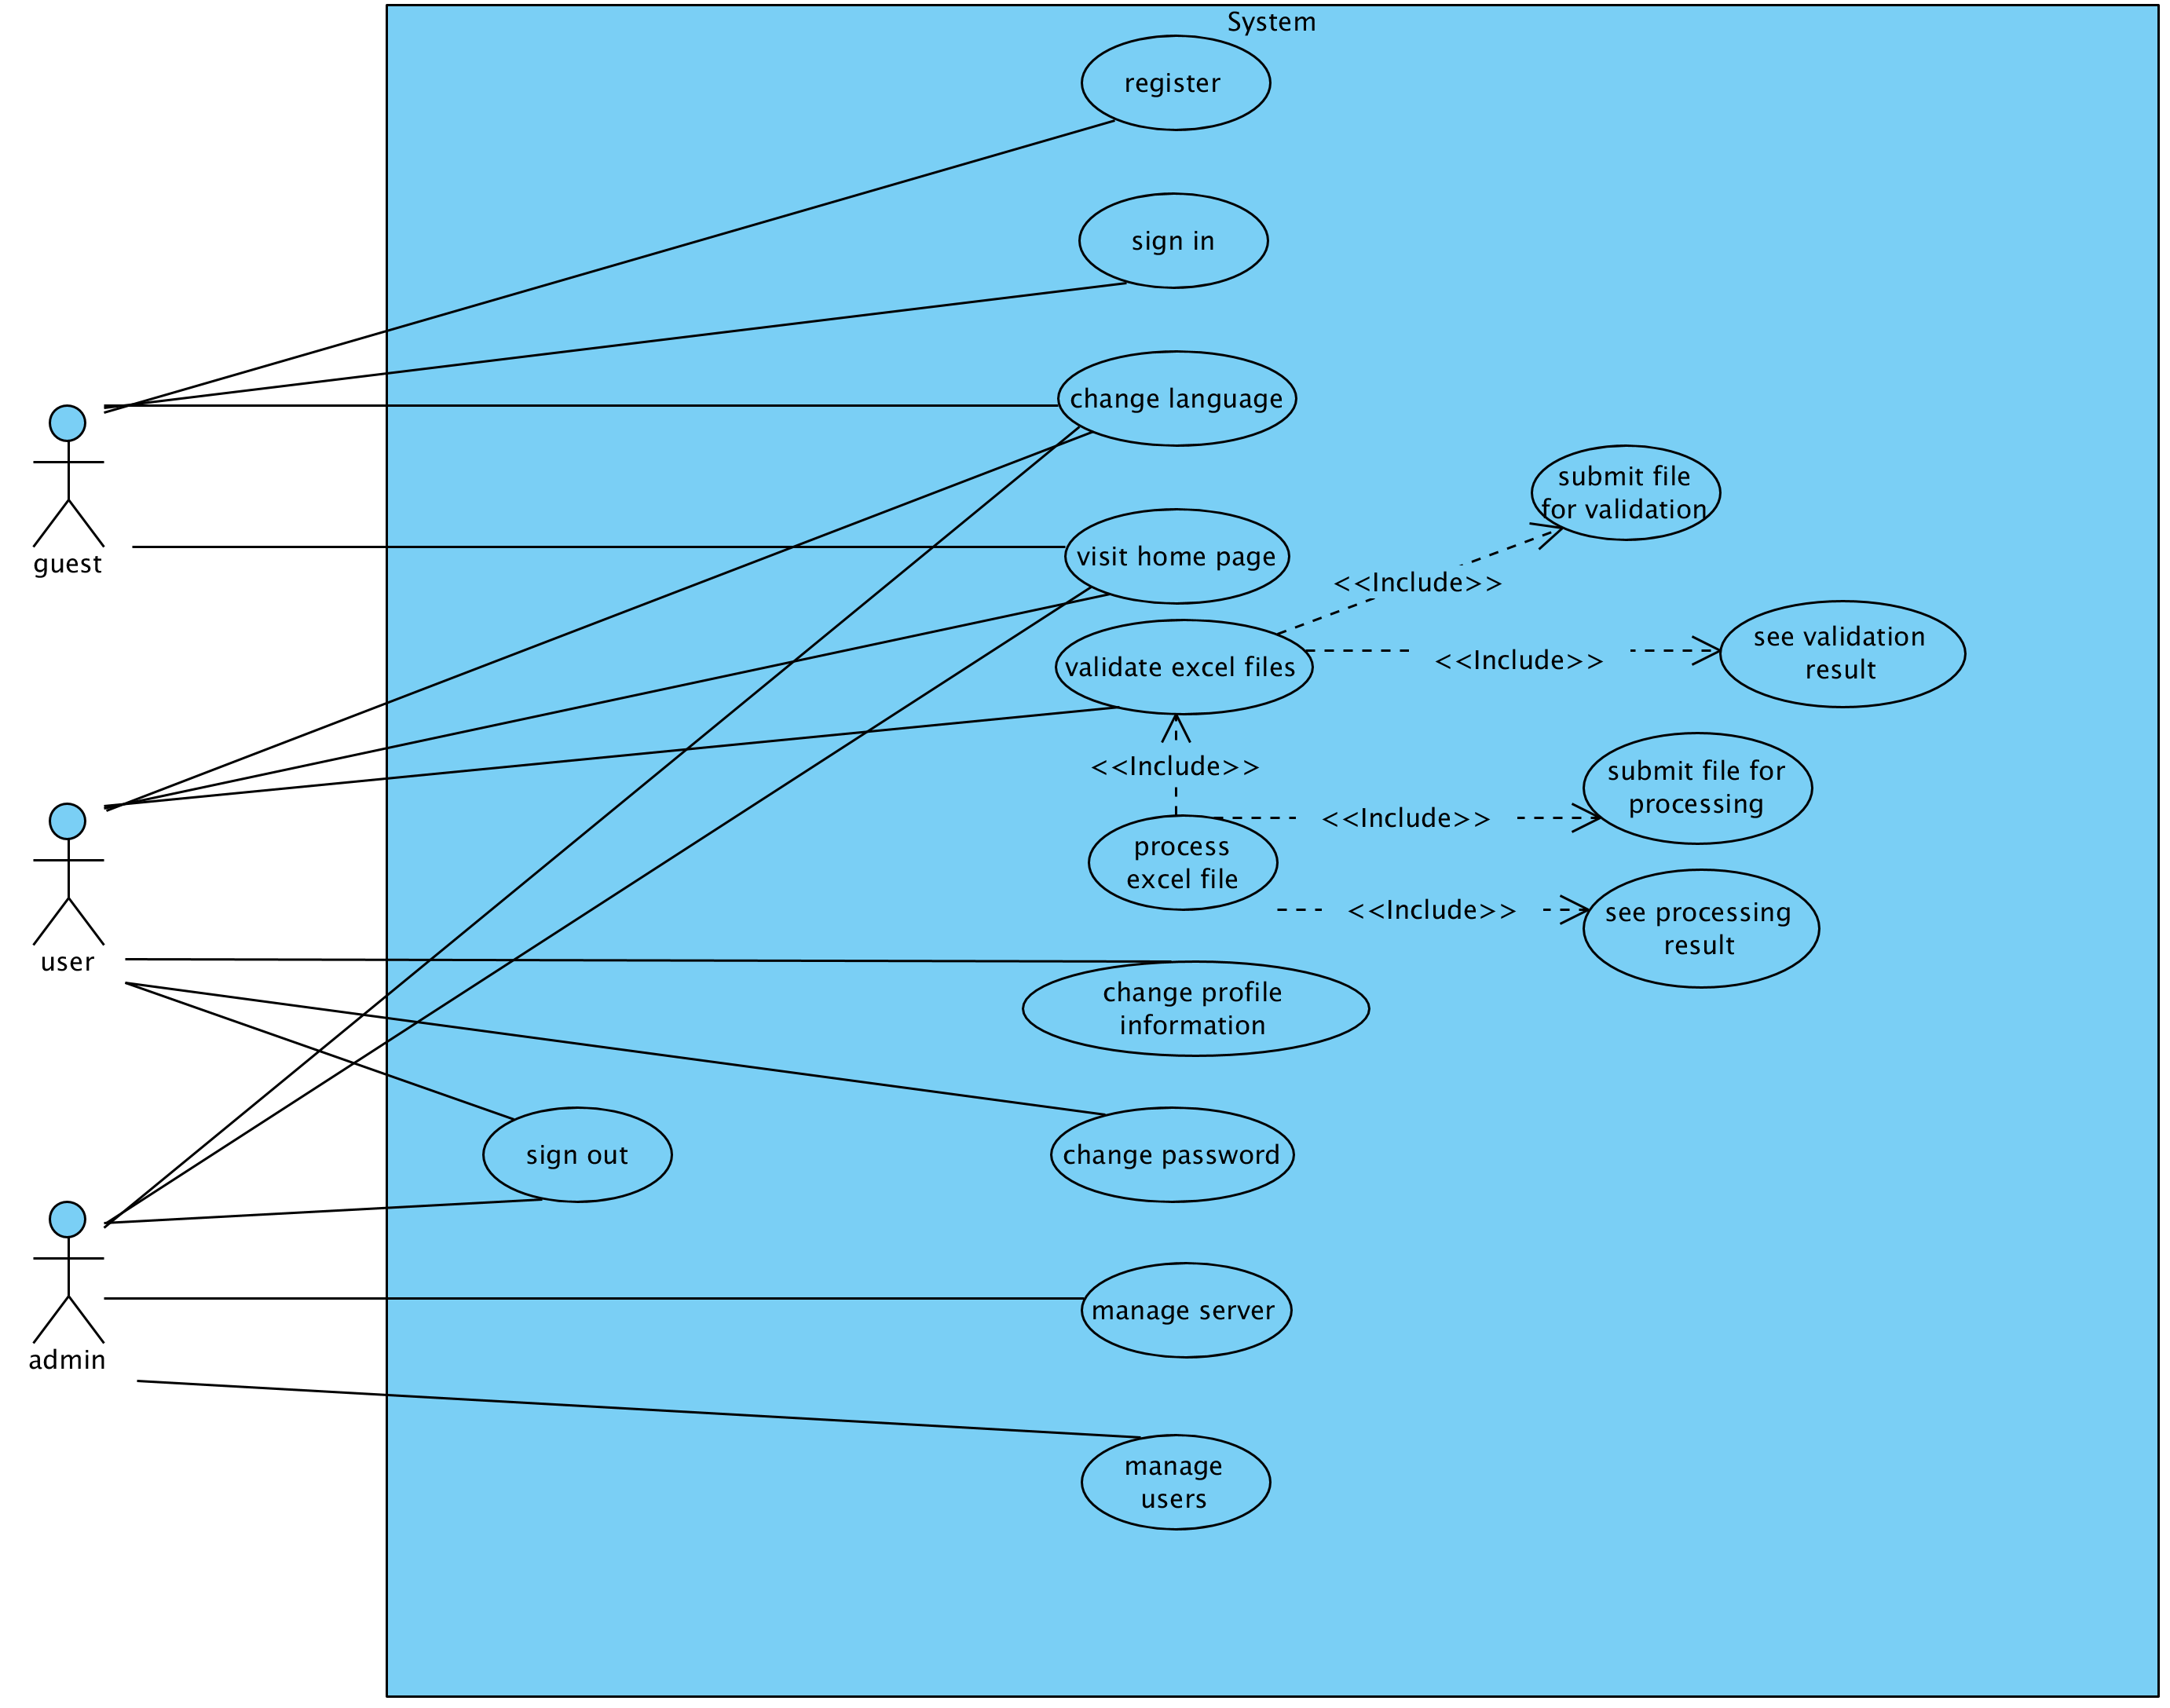
\includegraphics[width=0.8\textwidth]{images/diagrams/use-cases-macro.png}
    \caption{Les cas d'utilisation}
    \label{fig:use-cases-macro}
\end{figure}

\paragraph{}
Le diagramme \ref{fig:use-cases-macro} liste les différents cas d'utilisation et en l'analysant avec attention, on peut observer certains faits qui sont à première vue contre intuitifs.

\paragraph{}
Dans de nombreuses applications, on pourrait considérer une sorte d'héritage entre les différents niveaux de privilèges parmi les utilisateurs. Hors, ce n'est pas le cas ici. En effet, seul le \textbf{visiteur} a accès aux fonctionnalités pour s'enregistrer et se connecter. Plus surprenant, l'\textbf{administrateur} n'a pas accès aux fonctionnalités du coeur de l'application que sont la validation et le traitement des classeurs Excel. Encore plus étonnant, l'administrateur ne peut n'y accéder à son profil, n'y changer son mot de passe.

\begin{figure}[ht]
    \centering
    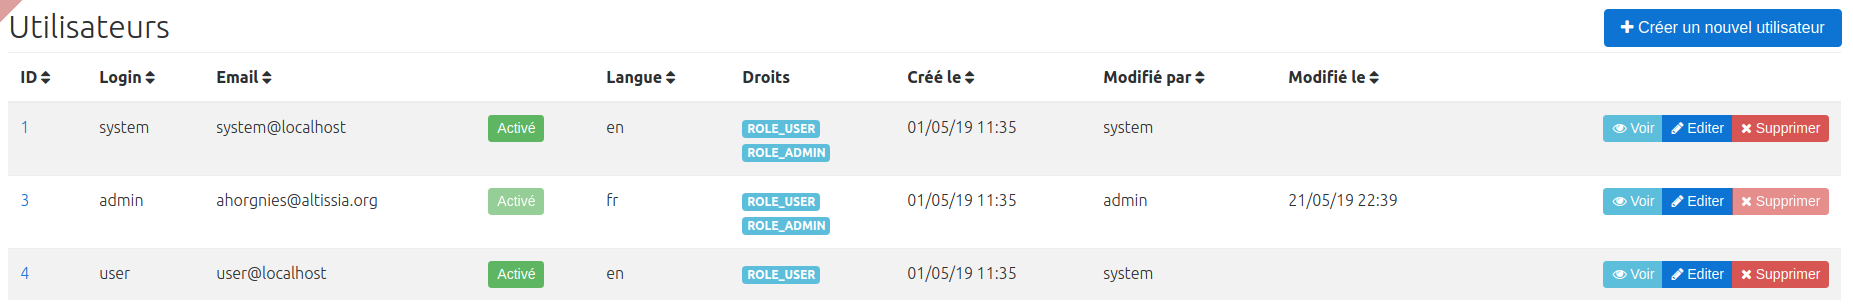
\includegraphics[width=0.8\textwidth]{images/screenshot/screenshot-user-admin-page.png}
    \caption{Une capture d'écran de la page de gestion des utilisateurs}
    \label{fig:user-admin-page}
\end{figure}

\paragraph{}
Cela est du au fait que les permissions sont gérées par un système de licences. Une personne peut cumuler les licences. Ainsi, plutôt que de faire hériter un rôle d'un autre, nous avons choisis de lier les permissions aux licences et de donner autant de licences que nécessaires aux personnes. Cela permet une gestion plus fine des autorisations et aussi plus simple à mettre en place.

Grâce à cela, la nouvelle application peut être déployé avec la base des utilisateurs existante complète sans risquer de compromettre les ressources qu'elle expose. En effet, seuls les personnes qui recevront la licence appropriée auront réellement accès à l'application.

De ce fait, un \textbf{visiteur} n'est pas une personne sans licence mais une personne qui n'a aucune licence adaptée.

Dans les faits, un \textbf{administrateur} aura toujours la licence d'un \textbf{utilisateur}. C'est ce que l'on peut observer sur l'image \ref{fig:user-admin-page}. Il a donc la double casque d'\textbf{administrateur} et d'\textbf{utilisateur}.

\paragraph{}
Le traitement inclue la validation. Bien que ces deux fonctionnalités soient fondamentalement distinctes, nous avons fait le choix d'inclure la validation comme première étape du traitement. Faire ainsi permet d'assurer la validité des données traitées et exclut toute erreur humaine.

\paragraph{}
Une chose qu'il n'est pas possible de voir sur ce diagramme \ref{fig:use-cases-macro} est que la validation et le traitement des classeurs sont des cas d'utilisation abstraits. En effet, il est nécessaire de les spécialiser sans quoi ils ne représentent rien.

Il faut se pencher sur des schémas plus détaillés pour comprendre ce que ces cas d'utilisation couvrent. C'est le sujet de la sous-section \ref{subsec:spreadsheet-use-case}.


\subsection{L'authentification}
\label{subsec:auth-feature}

\paragraph{}
L'authentification mise en place doit être compatible avec le système d'authentification présent sur les services d'Altissia. C'est particulièrement facile car c'est une authentification dite sans serveur. Cela veut dire qu'un client peut prouver son identité sans qu'un serveur tiers confirme les droits auxquels le \gls{g-client} prétend. 

\begin{figure}[h]
    \centering
    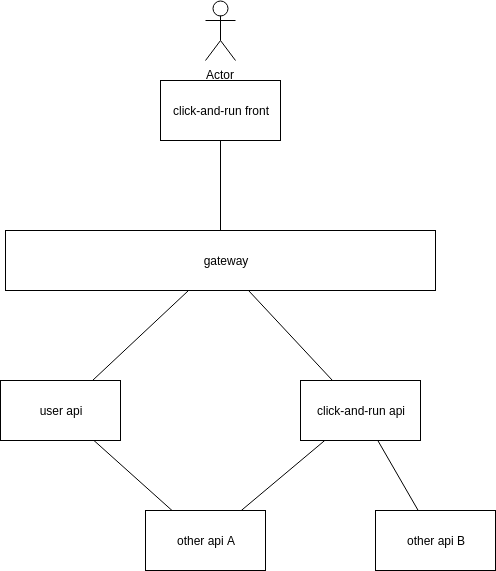
\includegraphics[width=0.7\textwidth]{images/diagrams/gw-archi.png}
    \caption{L'organisation des services et leurs communications (non \gls{a-uml})}
    \label{fig:gw-archi}
\end{figure}

\paragraph{}
Pour comprendre comment c'est possible, il faut d'abord s'intéresser à la manière dont les différents services communiquent entre eux. Comme on peut le voir sur le diagramme \ref{fig:gw-archi}, tous les \glspl{g-server} sont cachés derrière un unique point d'entrée que l'on appelle la passerelle. La passerelle vérifie que les demandes faites aux \glspl{g-server} sont authentifiées. Les demandes faites entre \glspl{g-server} ne sont pas vérifiées car les \glspl{g-server} se font mutuellement confiance.

\begin{figure}[h]
    \centering
    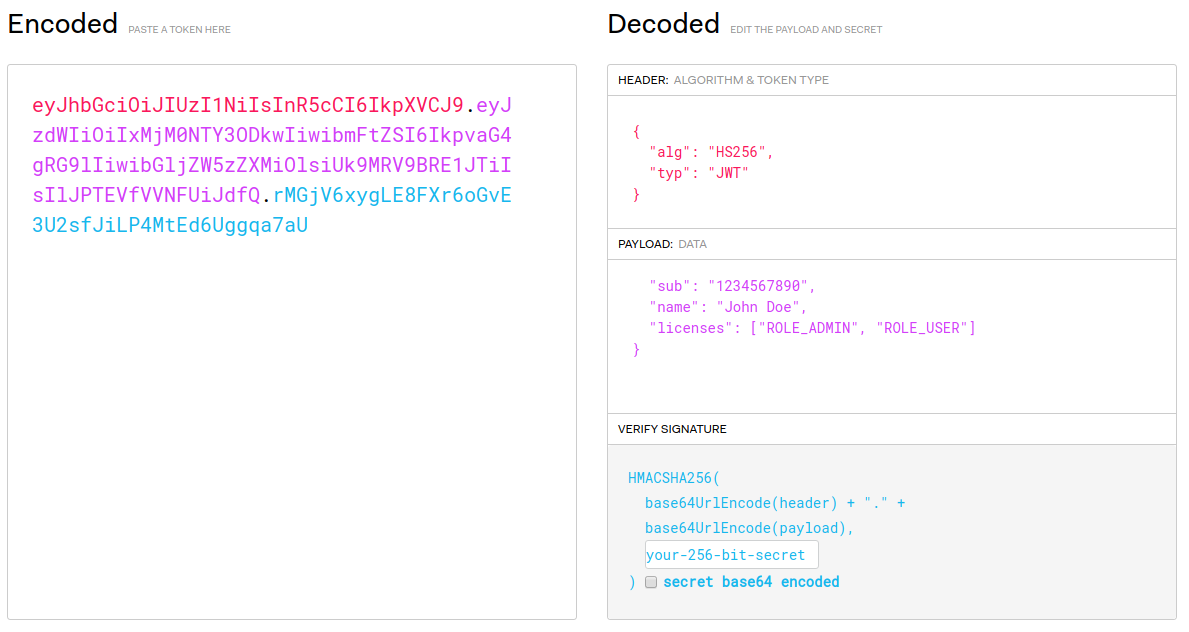
\includegraphics[width=0.7\textwidth]{images/screenshot/jwt-good-secret.png}
    \caption{Un \gls{a-jwt} à gauche et les données décodées à droite}
    \label{fig:jwt-good}
\end{figure}
\begin{figure}[h]
    \centering
    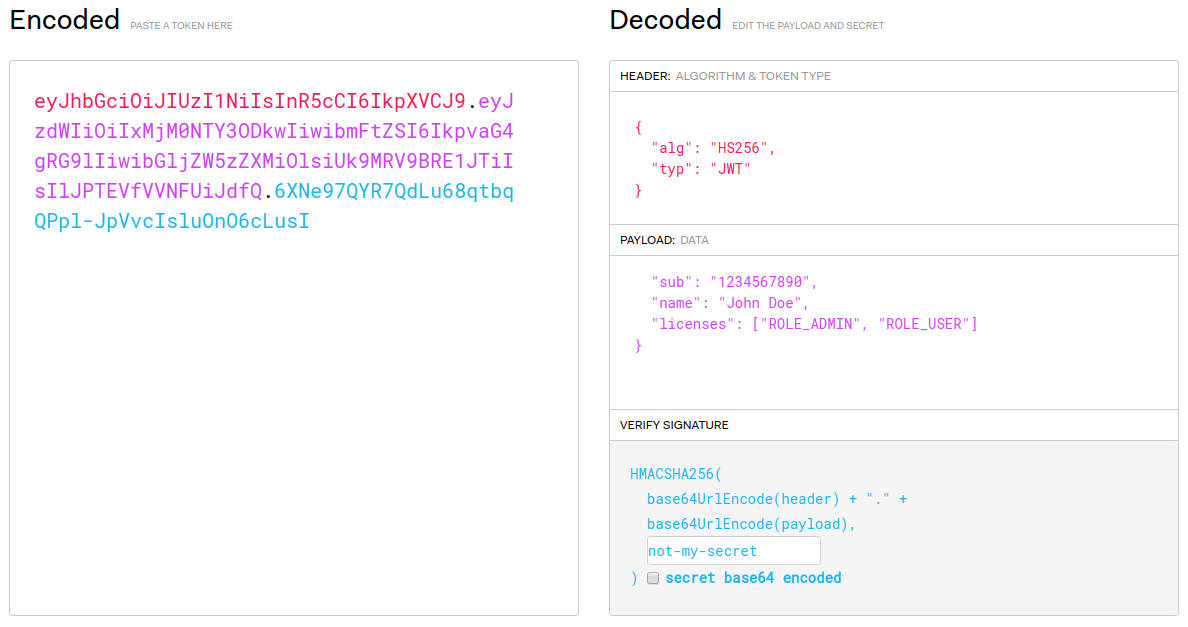
\includegraphics[width=0.7\textwidth]{images/screenshot/jwt-bad-secret.png}
    \caption{Un \gls{a-jwt} avec les mêmes données que sur la figure \ref{fig:jwt-good} mais pas la même signature}
    \label{fig:jwt-bad}
\end{figure}

\paragraph{}
Un \gls{g-client} qui veut s'authentifier fait sa demande à la passerelle.
La passerelle consulte le service des utilisateurs et si l'identifiant et le mot de passe concordent, elle approuve l'authentification.
Elle envoie alors un \gls{a-jwt}, dont on peut observer un exemplaire sur la figure \ref{fig:jwt-good} qui est une sorte de passeport qui déclare l'identité et les droits de l'utilisateur.
Ce \gls{a-jwt} est lisible par tous et est infalsifiable. Son contenu est accompagné d'une signature qui est la résultat de ce même contenu passé par une \gls{g-hash-func}.
La seule manière de reproduire cette signature est disposer de la \gls{g-hash-func} et du secret.
La figure \ref{fig:jwt-bad} illustre ce que l'on obtient sans le bon secret.
Cette formule est présente sur le \gls{a-jwt} et est donc accessible à tous.
Le secret lui n'est connu que par la passerelle et il n'y a donc que elle qui peut produire cette signature.

\paragraph{}
A chaque requête, un client accompagne sa demande de son \gls{a-jwt} et la passerelle reproduit la signature.
Si la signature produite est la même que celle inscrite sur le \gls{a-jwt}, la passerelle transmet la demande, sinon elle la rejette.
Et lorsque les \glspl{g-server} doivent communiquer entre eux pour remplir la demande du client, ils font confiance aux droits indiqués car ils ont été vérifiés par la passerelle.

\paragraph{}
Pour que cela fonctionne, la nouvelle application cliente doit:
\begin{enumerate}
    \item Adresser toutes ses demandes à la passerelle
    \item Implémenter la demande d'authenfication
    \item Fournir le \gls{a-jwt} à chaque requête
\end{enumerate}
Tandis que le nouveau \gls{g-server} doit juste contrôler que les droits d'un utilisateur correspondent au niveau d'autorisation requis pour les ressources qu'il demande.


\subsection{L'internalisation}
\label{subsec:i18n}

\paragraph{}
Chaque valeur textuelle statique\fnmark{} doit être traduite. Seuls des employés d'Altissia auront accès à cette application, il n'est donc pas nécessaire de traduire l'application dans toutes les langues supportées par les autres application d'Altissia\fnmark{}.
\fntext{Toutes données qui ne viennent pas d'une base de données sont dites statiques car elles ne peuvent pas changer pendant la vie de l'application.}
\fntext{Ce qui aurait fait une trentaine de langue dont je n'en connais que trois...}

Il est par contre obligatoire d'être compatible avec le système de localisation qui est déjà mis en place.

Altissia embarque les mécanismes nécessaires à la localisation dans chaque application. Une application peut donc changer de langue sans contacter de \gls{g-server}.

De plus, les informations de localisations sont stockées sur l'application web PhraseApp.
Les localisations devront donc être téléchargées depuis cette dernière.
Le format privilégié pour les applications clientes est le format \gls{a-json}, que l'application devra donc utiliser.

\paragraph{}
L'application cliente devra donc implémenter la localisation seule. C'est le sujet qui est abordé dans la sous section \ref{subsec:i18n-imp}


\subsection{La validation et le traitement des classeurs}
\label{subsec:spreadsheet-use-case}
TODO
